\documentclass[a4paper]{article}
\usepackage[a4paper,%
    text={180mm, 260mm},%
    left=15mm, top=15mm]{geometry}
\usepackage[utf8]{inputenc}
\usepackage{cmap}
\usepackage[english, russian]{babel}
\usepackage{indentfirst}
\usepackage{amssymb}
\usepackage{amsmath}
\usepackage{mathtools}
\usepackage{tcolorbox}
\usepackage{import}
\usepackage{xifthen}
\usepackage{pdfpages}
\usepackage{transparent}
\usepackage{graphicx}
\graphicspath{ {./figures} }

\newcommand{\incfig}[1]{%
\def\svgwidth{\columnwidth}
\import{./figures/}{#1.pdf_tex}
}

\begin{document}
\title{ТВиМС. Лекция}
\maketitle

\section*{\centering Двухфакторный дисперсионный анализ}

\begin{figure}[!htp]
    \begin{center}
        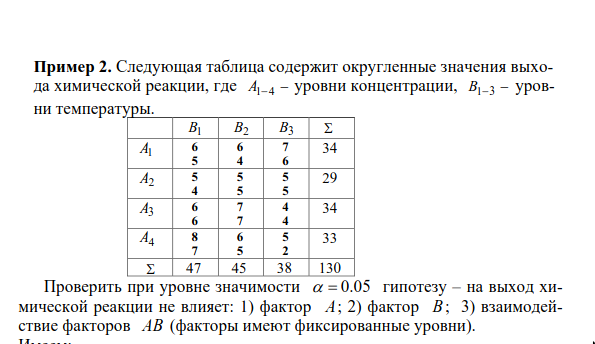
\includegraphics[width=0.95\textwidth]{tp-pic1.png}
    \end{center}
\end{figure}

A, B - факторы
\[
    m = 4 \ k = 3, \ n = 2 - \text{ число наблюдений в клетке}
\]
\[
    x_{ijl} \text{ - наблюдения} \quad x_{111} = 6, x_{112} = 5, \dots
\]
\[
    \overline{x}_{\dots} = \frac{\sum_{i=1}^{m}\sum_{j=1}^{k}\sum_{l=1}^{n} x_{ijl} }{} =
    \frac{130}{24} = 5.42
\]
\[
    Q = \sum_{i=1}^{m} \sum_{j=1}^{k} \sum_{l=1}^{n} (x_{ijl} - \overline{x}_{\dots})^2
\]
\[
    Q_{A} = kn \sum_{i=1}^{m} (x_{i..} - \overline{x}_{\dots})^2
\]
\[
    Q_{B} = mn \sum_{j=1}^{m} (x_{.j.} - \overline{x}_{\dots})^2
\]


\end{document}
